% ----------------------------------------------------------
\chapter{RESULTADOS}
% ----------------------------------------------------------


Esta seção tratará dos resultados obtidos, com a implementação da metodologia proposta no Capítulo 3, adaptações que precisaram ser feitas, e observações com relação ao modelo desenvolvido por Zhang et al. (2020a).
Antes da implementação integral de todos os submodelos, cada submodelo, mecânico e elétrico,  foi validado de forma separada. Dessa forma, foi possível ter um controle maior sobre cada operação. Cada submodelo foi validado com os resultados obtidos de Zhang et al. (2020a). Além dessa validação independente, uma validação da junção do modelo mecânico e elétrico, mas sem o termodinâmico, foi feita.
A implementação integral dos três submodelos apresentados não é uma validação, tendo em vista que os mesmo submodelos que Zhang et al. (2020a) utilizou não foram todos aplicados neste trabalho. Contudo, é possível fazer uma comparação dos resultados para perceber se há coerência no resultado final.   
	
\section{VALIDAÇÃO DO SUBMODELO ELÉTRICO}
				
Para a validação deste submodelo foi resolvida a Equação \ref{eq:eletrico} pelo método de Runge-Kutta de quarta ordem. Dados de entrada nesse modelo são os valores de $R$, $L$, $C$, $V_e$ e por fim $u_{emf}$, com isso a resolução do sistema retorna o valor de $I(t)$ em função do tempo.

Observações foram feitas com relação ao valor do fator de motor,  = 75 $NA{-1}$, dado na Tabela \ref{tab:Tab_1}, e foi percebido uma certa inconsistência no valor fornecido. 
%Pode-se ver na Figura \ref{fig:comp_e_75} uma comparação entre os resultados de Zhang et al. (2020a) e aqueles obtidos no presente trabalho. 
Convém ressaltar que foi feita uma verificação do método Runge-Kutta comparando-o com uma rotina pré-existente no Matlab. 



% \begin{figure}[htb]
%	\caption{\label{fig:comp_e_75}Comparação das curvas para o submodelo elétrico tendo como referência Zhang et al. (2020a). Discrepância entre os resultados para  = 75 NA-1.}
%	\begin{center}
%		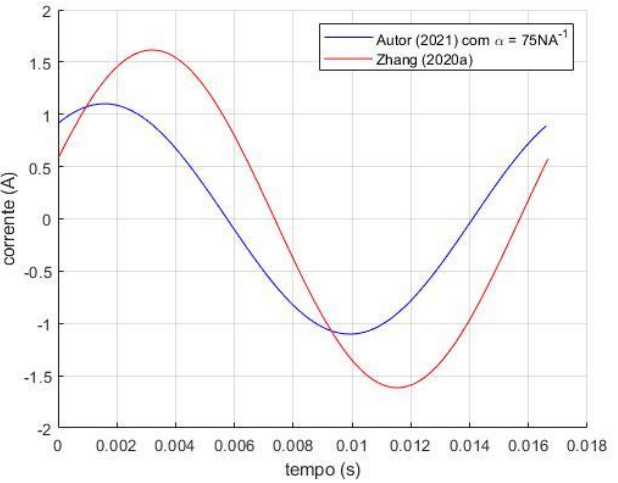
\includegraphics[scale=0.6]{images/e_75.png}
%	\end{center}
%	\fonte{Autor (2021)}
%\end{figure}

Para resolver esse problema, tentou-se contatar sem sucesso os autores do referido trabalho a fim de verificar um possível erro tipográfico no artigo. Posteriormente, vários valores de  foram testados como entrada, até que se percebeu um padrão na movimentação da curva resultante. Dessa forma, foi encontrado um valor em que a resposta se justapõe muito bem na curva de referência. No caso, o valor encontrado foi de  = 35 $NA^{-1}$, e a nova comparação pode ser vista na Figura \ref{fig:comp_e_35}. Sabe-se que o valor encontrado pode não ser correto, e com isso não ter um resultado correto, porém adotou-se esse valor para que futuramente esse dado possa ser encontrado 




 \begin{figure}[h]
	\caption{\label{fig:comp_e_35}Comparação das curvas para o submodelo elétrico tendo como referência Zhang et al. (2020a). Concordância entre os resultados para  = 35 NA-1.}
	\begin{center}
		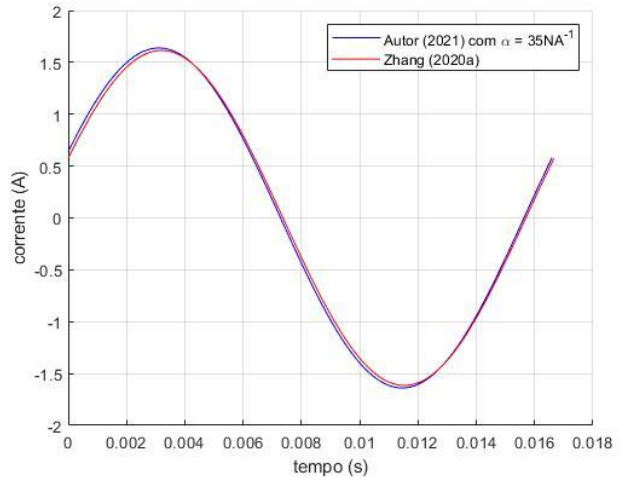
\includegraphics[scale=0.55]{images/e_35.png}
	\end{center}
	\fonte{Autor (2021)}
\end{figure}

A curva da Figura \ref{fig:comp_e_35}, apresenta os dois resultados praticamente iguais. Com esse resultado, assume-se que esse submodelo fornece resultados que são coerentes, visto que se aproximou do resultado de Zhang et al. (2020a), apesar da inconsistência encontrada no fator de motor. 
\vfill

\section{VALIDAÇÃO DO SUBMODELO MECÂNICO}

Para a validação do submodelo mecânico foi resolvida a Equação \ref{eq:mecanico} pelo método de Runge-Kutta de quarta ordem. Dados de entrada nesse modelo são os valores de $m_{eff}$, $k_s$, $c_{fri}$, $P_{shell}$, $P(t)$, $A_p$, $\alpha$ e por fim $I(t)$, com isso a resolução do sistema retorna o valor de $x_p(t)$ em função do tempo.

Na etapa da validação do submodelo mecânico, assim como o submodelo elétrico,  Zhang et al. (2020a) não divulgaram o valor do coeficiente de fricção, $c_{fri}$. Por consequência, dados sobre coeficiente de fricção em compressores lineares foram pesquisados. Na tese de doutorado de Bradshaw (2012), sobre um modelo miniatura de um compressor linear para arrefecimento de eletrônicos, o autor comenta que utiliza valores entre 0,1 e 0,3 kg/s em seu trabalho.

Dessa forma, foram adotados como possíveis valores: 0,1, 0,2 e 0,3 kg/s. Ao aplicar esses valores no código não houve diferença perceptível em relação ao resultado, porém percebeu-se que quanto maior o valor de $c_{fri}$ mais rápido a simulação atinge uma condição de regime periódico. Além disso, embora os autores tenham fornecido as massas do pistão e das molas, eles não indicaram a massa móvel efetiva do sistema. Como uma primeira tentativa, optou-se por calcular a massa efetiva como $m_{eff}=m_p+1/3m_s$, onde $m_p$ é a massa do pistão e ms é a massa das molas, conforme sugerido por Rao (2018). %A Figura \ref{fig:m_13} é o resultado do submodelo mecânico para $m_{eff}=m_p+1/3m_s$, e é representada num gráfico de deslocamento por tempo. 

 % \begin{figure}[htb]
%	\caption{\label{fig:m_13}Comparação do deslocamento por tempo para com o submodelo mecânico, tendo massa efetiva do sistema igual a $m_{eff}=m_p+1/3 ; m_s=0.6867$ kg com o resultado de Zhang et al. (2020).}
%	\begin{center}
%		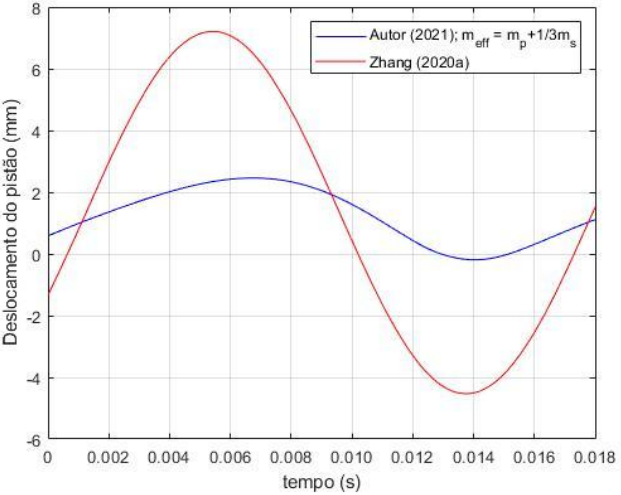
\includegraphics[scale=0.65]{images/m_13.png}
%	\end{center}
%	\fonte{Autor (2021)}
%\end{figure}


%Analisando a Figura \ref{fig:m_13} é possível observar a comparação entre deslocamento no pistão para meff=mp+1/3ms e a referência. A amplitude do deslocamento é relativamente menor que de Zhang et al. (2020a), não sendo um valor aceitável para uma validação.Dentre as alternativas para contornar esse problema, a que mais fez sentido, foi ajustar o valor da massa efetiva, visto que não foi fornecida. Dessa forma escolheu-se a como a massa efetiva a própria massa do pistão, porém os resultados também não foram aceitáveis, a Figura \ref{fig:comp_m_orig2} mostra o resultado da simulação com $m_{eff}=m_p =0,632 kg$.
 
	
% \begin{figure}[htb]
%    \caption{\label{fig:comp_m_orig2}Comparação das curvas para com o submodelo mecânico, tendo massa efetiva do sistema igual a $m_{eff}=0,632 kg$}
%    \begin{center}
%	    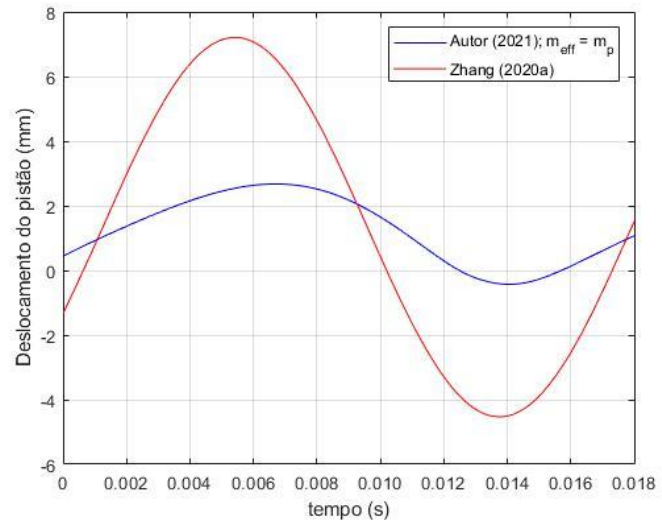
\includegraphics[scale=0.65]{images/m_p.png}
%    \end{center}
%    \fonte{Autor (2021)}
%\end{figure}


%A Figura \ref{fig:comp_m_orig2} assim como a \ref{fig:m_13} comparam o deslocamento do pistão em relação a Zhang et al. (2020a). Os dois resultados tiveram resultados próximos pelo motivo da massa efetiva não variar significativamente. De certa forma, era esperado um resultado não muito diferente em relação ao anterior. 
Tendo resultados para $m_{eff}$ não aceitáveis com o método dito, decidiu-se encontrar uma massa efetiva que aproximasse os resultados. Então, foi adotado $m_{eff}$ =0,400 kg. É entendido que este é um valor irreal, pois a massa mínima esperada seria o peso do pistão, contudo isso é um ponto a ser melhorado em trabalhos futuros. Os resultados de deslocamento do pistão são comparados na Figura \ref{fig:comp_m_04}, que apresenta amplitudes aparentemente iguais, porém com fases um pouco diferentes. Supõe-se que esta defasagem seja um efeito combinado de incertezas associadas tanto à massa efetiva quanto ao coeficiente de fricção. Supõe-se que um ajuste melhor das curvas possa ser obtido variando estes dois parâmetros em um procedimento de otimização. Porém, considera-se que os resultados atuais já são suficientes para atender os objetivos do presente trabalho, sendo, portanto, adotados como valores de referência daqui pra frente.

 \begin{figure}[htb]
	\caption{\label{fig:comp_m_04}Comparação das curvas para com o submodelo mecânico, tendo massa efetiva do sistema igual a $me_{eff}=0,400kg$.}
	\begin{center}
		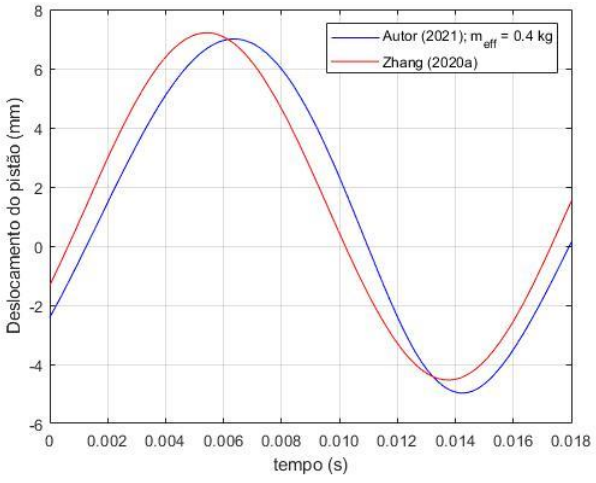
\includegraphics[scale=0.65]{images/m_04.png}
	\end{center}
	\fonte{Autor (2021)}
\end{figure}

%\section{VALIDAÇÃO DO MODELO ELETROMECÂNICO ACOPLADO}

%Com as validações apresentadas nas Seções 4.1 e 4.2, pode-se partir para validação da união dos dois submodelos. O resultado do deslocamento do pistão em função do tempo pode ser visto na Figura 15, onde é mostrada a oscilação resultante do pistão em regime periódico.


 %\begin{figure}[htb]
%	\caption{\label{fig:comp_e_m}Comparação do resultado que mostra o deslocamento pelo tempo da união dos submodelos mecânico e elétrico em relação a Zhang et al (2020a).}
%	\begin{center}
%		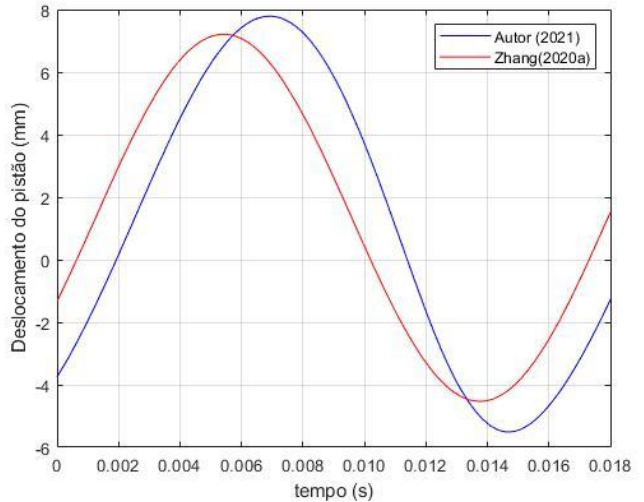
\includegraphics[scale=0.55]{images/e_m.png}
%	\end{center}
%	\fonte{\cite{bradshaw}}
%\end{figure}


%Analisando o acoplamento dos dois submodelos em relação ao deslocamento na Figura \ref{fig:comp_e_m}, é possível perceber uma pequena diferença em relação a validação do submodelo mecânico, isso acontece pelo fato de que no submodelo mecânico, os dados da corrente elétrica foram retirados dos resultados de Zhang et al. (2020a), não sendo afetados pela velocidade do pistão com a força eletromotriz inversa. Enquanto no acoplamento dos submodelos, a corrente já é calculada tendo como parâmetro de entrada a velocidade do pistão. Dessa forma, como já havia uma pequena discrepância nos resultados obtidos no submodelo mecânico, esse erro pode ter se propagado para a união dos submodelos.
%Para entender melhor o efeito percebido na Figura \ref{fig:comp_e_m}, os dados da corrente do modelo eletromecânico e do submodelo mecânico foram comparados em um gráfico pelo tempo. Tais dados são mostrados na Figura \ref{fig:comp_acopl}. 


 %\begin{figure}[htb]
%	\caption{\label{fig:comp_acopl}Comparação das curvas da corrente pelo tempo do submodelo eletromecânico acoplado com o submodelo mecânico.}
%	\begin{center}
%		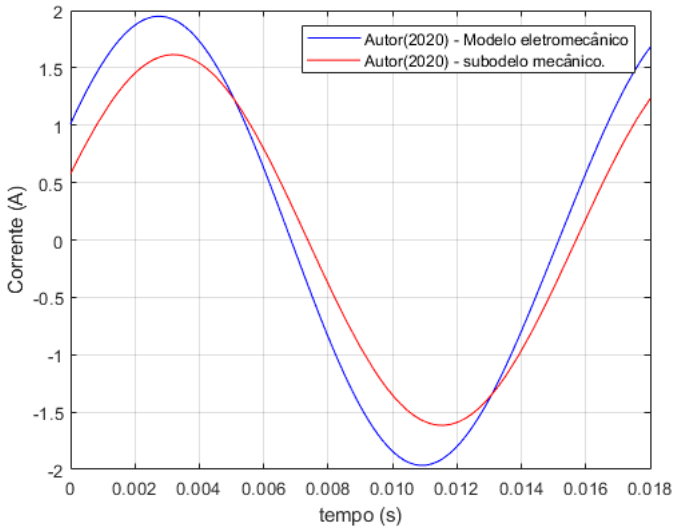
\includegraphics[scale=0.55]{images/c_e_m.png}
%	\end{center}
%	\fonte{\cite{bradshaw}}
%\end{figure}

%Percebe-se, na Figura \ref{fig:comp_acopl}, que existe uma variação da corrente entre os dois modelos, isto se deve pelo fato de no modelo eletrodinâmico a velocidade do pistão interferir na corrente com a força eletromotriz inversa, e no mecânico a corrente usada é o resultado de Zhang et al. (2020a), não sendo afetada pela velocidade do pistão.

\section{ACOPLAMENTO DO MODELO ELETROMECÂNICO COM O TERMODINÂMICO}

Toda a teoria apresentada, discutida e de certa forma validada foi necessária para ser aplicada nesta seção. Como comentado anteriormente, devido ao fato do modelo de Zhang et al. (2020a) e este desenvolvido não aplicarem os mesmos submodelos, não faz sentido validar o modelo aqui desenvolvido. Tendo isso em vista, ao invés de uma validação foi feita uma comparação com o modelo de Zhang et al. (2020a). Embora não se espere que os resultados obtidos sejam exatamente iguais, é possível compará-los a fim de verificar  a coerência física.
Esta seção mostra o resultado do acoplamento do modelo eletromecânico com o ciclo ideal de compressão do vapor. O resultado do deslocamento pelo tempo pode ser visto na Figura \ref{fig:comp_desloc}. Esses dados representam o deslocamento no centésimo ciclo, já em regime periódico. O deslocamento, na abscissa, dos dois modelos se apresenta próximo. 


 \begin{figure}[htb]
	\caption{\label{fig:comp_desloc}Comparação do resultado do deslocamento do pistão entre o modelo desenvolvido neste trabalho e ao modelo de Zhang et al (2020a).}
	\begin{center}
		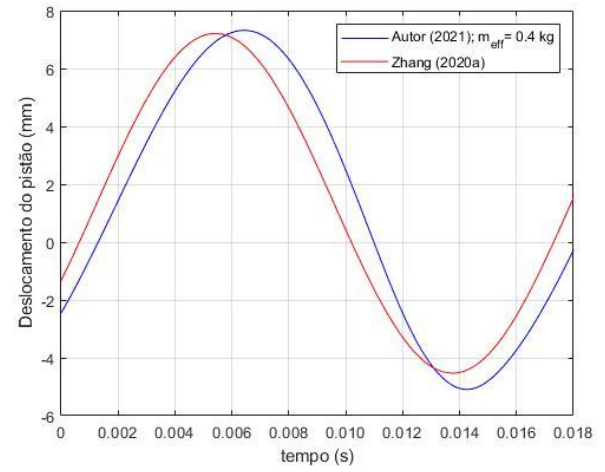
\includegraphics[scale=0.60]{images/e_m_t.png}
	\end{center}
	\fonte{Autor (2021)}
\end{figure}


%A Figura \ref{fig:comp_pres} compara a pressão na câmara de compressão do modelo desenvolvido com o resultado de Zhang et al. (2020) para o centésimo ciclo. Na Figura \ref{fig:comp_pres} ainda é possível observar os efeitos de vazamentos e a dinâmica de válvulas  não aplicadas no modelo.

% \begin{figure}[htb]
%	\caption{\label{fig:comp_pres}Pressão em função do tempo na câmara de compressão em comparação com a de Zhang et al. (2020).}
%	\begin{center}
%		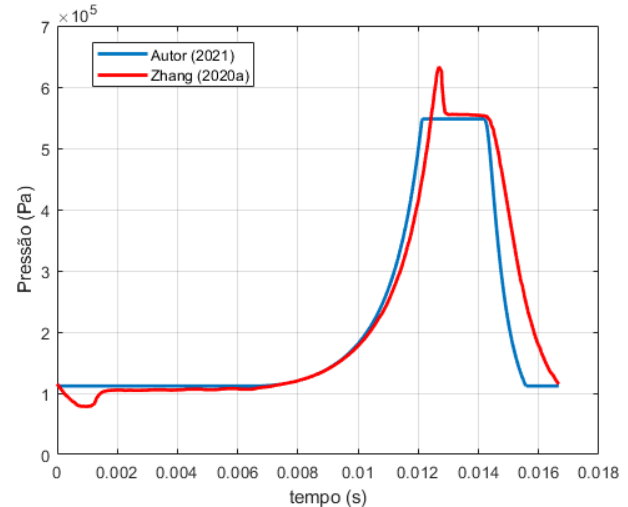
\includegraphics[scale=0.60]{images/pressao_zhang_02.png}
%	\end{center}
%	\fonte{Autor (2021)}
%\end{figure}


%A Figura \ref{fig:comp_pres} apresenta a pressão variando em função do tempo. Com isso, percebe-se, no modelo desenvolvido, que no instante 0,012 s a válvula de descarga é aberta mantendo a pressão constante até aproximadamente o instante 0,014. De fato, isso condiz com a Figura \ref{fig:comp_desloc}, no instante  0,012 s o pistão está chegando no TDC, comprimindo o fluido de trabalho. No instante 0,014 o deslocamento começa no sentido contrário, o que faz com que a válvula de descarga se feche e dessa forma diminuindo bruscamente a pressão.



 %\begin{figure}[htb]
%	\caption{\label{fig:comp_elet}Comparação do resultado mostrado em função das correntes pelo tempo entre o modelo desenvolvido neste trabalho e ao modelo de Zhang et al (2020a).}
%	\begin{center}
%		\includegraphics[scale=0.60]{images/c_c_zhang.png}
%	\end{center}
%	\fonte{Autor (2021)}
%\end{figure}

%A Figura \ref{fig:comp_elet} apresenta a comparação do resultado da corrente com o resultado de Zhang et al. (2020) para o centésimo ciclo. Comparando a Figura \ref{fig:comp_elet} com a do modelo eletromecânico, Figura 16, observou-se uma menor amplitude da corrente. Esse fato pode ser explicado pelo modelo eletromecânico comparado usar os dados da pressão de Zhang et al. (2020), enquanto o modelo da Figura \ref{fig:comp_elet} usa o ciclo ideal de compressão.

%É importante ressaltar que durante esta simulação observou-se que a força fictícia $F_a$, dada pela equação 7, foi ativada mesmo quando o sistema atinge a condição periódica. Isso se deve ao fato de que o carregamento dinâmico de pressão sobre o pistão foi alterado em relação ao resultado apresentado por Zhang et al. (2020a), uma vez que os submodelos termodinâmicos não são exatamente iguais.
\vfill


\section{ANÁLISE DA SENSIBILIDADE DO MODELO} 

Após as validações e comparações, nesta seção serão mostradas algumas análises feitas, entre elas: eficiências mecânica e elétrica em função da variação da razão de pressão, PR, variação das potências mecânica e elétrica em função da razão de pressão e uma análise da transmissibilidade do pistão.
Na Figura \ref{fig:comp_PR_efic}, é possível observar como as eficiências variam de acordo com a razão de pressão. Observa-se que a eficiência mecânica tende a aumentar enquanto que a eficiência elétrica sofre menos variações. Percebe-se também que quando PR = 3,6, existe um aumento brusco de eficiência mecânica acompanhado de uma redução significativa de eficiência elétrica, porém, não foi entendido o porquê desse comportamento. Simulações adicionais, além dos pontos mostrados na Figura \ref{fig:comp_PR_efic}, realizadas com PR próxima a 3,6 indicam que realmente existe um ponto ótimo de eficiência elétrica nessa região.  


 \begin{figure}[htb]
	\caption{\label{fig:comp_PR_efic} Análise de diferentes razões de pressões e seu efeito nas eficiências.}
	\begin{center}
		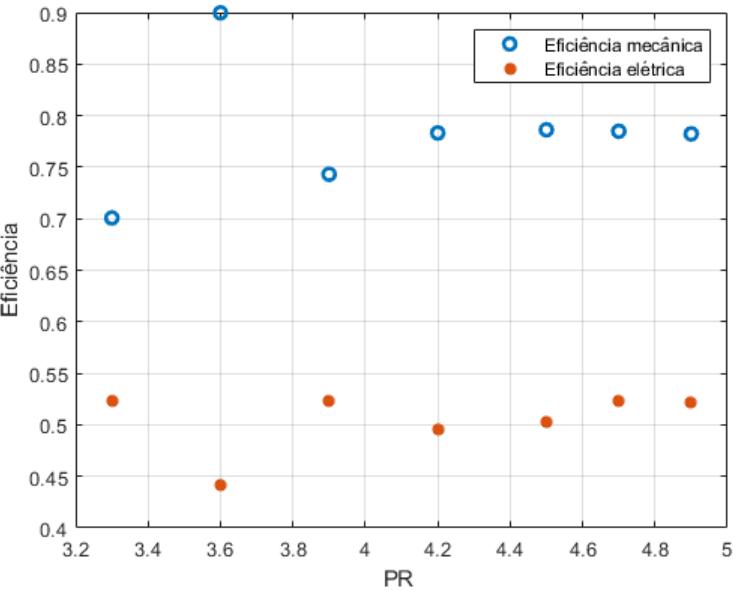
\includegraphics[scale=0.50]{images/efic.png}
	\end{center}
	\fonte{Autor (2021)}
\end{figure}




Na Figura \ref{fig:comp_PR_pot} encontram-se as potências em cada etapa: potência elétrica, potência mecânica, e potência termodinâmica. Percebe-se que, de fato, a potência elétrica consumida quando PR = 3,6 assume um mínimo e que mesmo que a potência mecânica também seja menor, a queda brusca da potência elétrica justifica o aumento da eficiência elétrica. Sendo assim, em trabalhos futuros será conveniente entender as razões que levam a essa condição de potência elétrica. 

 \begin{figure}[htb]
	\caption{\label{fig:comp_PR_pot}Análise do efeito da variação da razão de pressões nas potências elétrica, mecânica e termodinâmica.}
	\begin{center}
		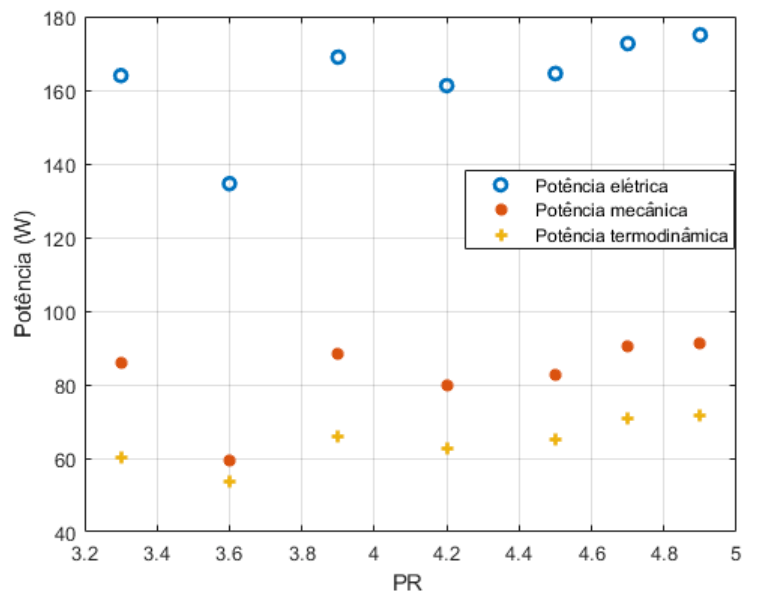
\includegraphics[scale=0.50]{images/pote.png}
	\end{center}
	\fonte{Autor (2021)}
\end{figure}

\nocite{anuario}
\nocite{bijanzada}
\nocite{bijanzadb}
\nocite{bradshaw}
\nocite{coolprop}
\nocite{coulomb}
\nocite{liang}
\nocite{oliveira}
\nocite{ono}
\nocite{pdsim}
\nocite{rao}
\nocite{refrigeration-ademe}
\nocite{silva}
\nocite{webplot}
\nocite{zhanga}
\nocite{zhangb}
